%!TEX root = ../template.tex
%%%%%%%%%%%%%%%%%%%%%%%%%%%%%%%%%%%%%%%%%%%%%%%%%%%%%%%%%%%%%%%%%%%%
%% chapter4.tex
%% NOVA thesis document file
%%
%% Chapter with lots of dummy text
%%%%%%%%%%%%%%%%%%%%%%%%%%%%%%%%%%%%%%%%%%%%%%%%%%%%%%%%%%%%%%%%%%%%

\typeout{NT FILE chapter4.tex}%

\chapter{Work Plan}
\label{cha:work_plan}

We have divided the work to be done into the following tasks, which are depicted in Figure ~\ref{fig:gantt}:

\begin{itemize}
    \item \textbf{Development of the compatibility verification procedure:} This task consists on the implementation of the compatibility verification procedure that compares OpenAPI contracts.
    \item \textbf{Development of the service registry:} This task entails designing and implementing the service registry.
    \item \textbf{Development of the adapter proxy:} This task entails designing and implementing the adapter proxy.
    \item \textbf{Development of the benchmark platform:} This task involves writing load testing, argo, prometheus, and kubernetes scripts to support the benchmark platform, as well as a bash script that acts as an interface to the platform.
    \item \textbf{Development of the benchmark target solutions:} This task consists on the development of the various solutions to the evolution of contracts in microservices.
    \item \textbf{Experimental evaluation:} This will consist on the setup of kubernetes cluster and the evaluation of each solution granularity, terminal, type, scalability, maintainability and performance via the benchmark platform and empirical evidence.
    \item \textbf{Writing of the dissertation document:} This task involves on the continuous writing of the dissertation, which
    will be done in parallel with the other activities.
\end{itemize}

\begin{figure}[htbp]
    \centering
    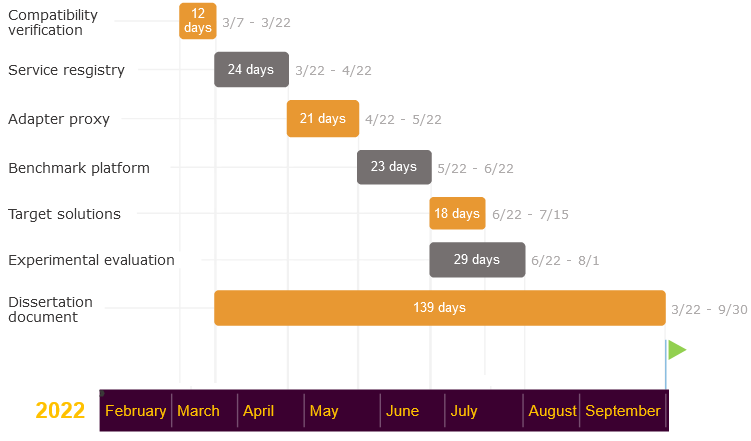
\includegraphics[height=4in]{gantt}
    \caption{Proposed thesis work plan.}
    \label{fig:gantt}
\end{figure}
